\documentclass{article}
\usepackage{mathrsfs}
\usepackage{amsmath}
\usepackage{mathtools}
\usepackage{graphicx}
\DeclarePairedDelimiter{\ceil}{\lceil}{\rceil}


\begin{document}
\begin{center}
\textbf{\huge{Week 6}}
\end{center}

\section{Random variable source coding}

Let $\underbar{c}(x)$ be the codeword assigned to $x \in \mathcal{X}$.

$l(x)$ be the length of codeword assigned to $x$.

Here we are coding a single random variable and all codewords are binary strings. (Fixed-variable length source coding)
$$ \mathscr{C}= \{ \underbar{c}(x): x \in \mathcal{X}\}$$

$$ L_{\mathscr{C}}= \sum_{x \in \mathcal{X}}p(x)l(x)$$

Our goal is to design a code which has minimum $L_{\mathscr{C}}$, $L^{*}$
$$L^{*} = \text{min}_{\mathscr{C}} L_{\mathscr{C}}$$

\subsection{Kraft inequality}

Let $\mathscr{C}$ be any prefix-free (binary) code. Then,
$$ \sum_{x \in \mathcal{X}} 2^{-l(x)} \leq 1$$

Proof: We know that any prefix-free code can be represented using a binary tree which has `leaves' as the codeword. In the binary tree corresponding to the code, the depth of the tree would be the length of the largest codeword in the code. ($l_{\text{max}}=max_{x \in \mathcal{X}} l(x)$)\\

Suppose there is a codeword $\underbar{c}$ of length $l$ represented by a node at depth l($l \leq l_{\text{max}}$).\\

Then $\underbar{c}$ has $2^{l_{\text{max}}-l}$ successors at level $l_{\text{max}}$. Also, none of these are codewords as the code is prefix-free. Now,

\begin{align}
    \sum_{\underbar{x} \in \mathcal{X}} 2^{l_{\text{max}}-l(\underbar{x})} \leq 2^{l_{\text{max}}}
\end{align}
This is true if distinct codewords $\underbar{c1}$, $\underbar{c2}$ don't have common successors at $l_{\text{max}}$ level. Any successor of $\underbar{c1}$ at $l_{\text{max}}$ has $\underbar{c1}$ as a prefix. Similarly in the other case as well.

Suppose $l(\underbar{c1}) \leq l(\underbar{c2})$, so there can be a common successor $\underbar{v}$ at $l_{\text{max}}$.

Then, $\underbar{v}$ has first $l(\underbar{c1})$ places as $\underbar{c1}$ and first $l(\underbar{c2})$ places as $\underbar{c2}$.\\

$\Rightarrow$ $\underbar{c1}$ should be a prefix of $\underbar{c2}$ which isn't true as $\mathscr{C}$ is a prefix-free code. Hence, no pair of codewords in $\mathscr{C}$ have any common successors.

Hence $(1)$ is true. And dividing both sides by $2^{l_{\text{max}}}$ gives us the Kraft inequality.

\subsection{Lemma}
$$ L^{*} \geq H(X)$$
Any prefix-free code for $X$ has average length of at least $H(X)$.

Proof:
$$ L - H(X) =  \sum_{x \in \mathcal{X}}p(x)l(x) - \sum_{x \in \mathcal{X}} p(x) \log \frac{1}{p(x)}$$
We know,
 $$ D(p||q)= \sum_{x \in supp(P_X)}p(x)\log \frac{p(x)}{q(x)}$$
 Let
$$ q(x):= \frac{2^{-l(x)}}{\sum_{x \in \mathcal{X}} 2^{-l(x)}}   $$

\begin{align*}
    D(p_X || q_X) &= \sum_{x \in supp(P_X)}p(x)\log \frac{p(x)}{\frac{2^{-l(x)}}{\sum_{x' \in \mathcal{X}} 2^{-l(x')}}} \\
    &= - \sum p(x) \log \frac{1}{p(x)} + \sum p(x) \log \frac{1}{\frac{2^{-l(x)}}{\sum_{x' \in \mathcal{X}} 2^{-l(x')}}} \\
    &= -H(X) + \sum_{x \in supp(p_x)} p(x) \log 2^{l(x)} + \sum_{x \in supp(p_x)} p(x) \log \sum_{x'} 2^{-l(x')}  \\
    &= -H(X)+ L - \epsilon \qquad (\text{from Kraft's})\\
    & \leq - H(X)+L
\end{align*}
$$ \Rightarrow L_{\mathscr{C}} - H(X) \geq 0$$
 $$ L^{*} \geq H(X)$$

 Note: Equality happens only iff $p_x = q_x$ and $\epsilon$ is zero.
 %30/6
 \subsection{Lemma}
 Suppose we have a random variable $X \in \{ x_1, x_2, \cdots, x_k\}$ and positive integers such that $\sum_{i=1}^{k} 2^{-l_i} \leq 1$.

 Then there exists a prefix free code for $X$ with codeword lengths $l_1 , l_2 , \cdots, l_k$.\\

 Proof: We can construct a binary tree with leaves at depths $l_1, l_2, cdots, l_k$ such that none of these nodes are successors of each other, i.e. they are leaves of some binary tree (valid p-f code).

 Assume that $l_1 \leq l_2 \leq \cdots \leq l_k$, without loss in generality    , for any $i \leq k$,
 \begin{equation}
     \sum_{1}^{i-1} 2^{-l_i} <1
 \end{equation}

Imagine we take the full binary tree upto level $l_k$. At each step of the algorithm we intend to pick one available (undeleted) node from the above tree at level $l_i$ and delete all it's successors from the tree. Repeat this process for $i=1, \cdots , k$, we will then have a prefix-free tree.

We have to show that at each step $i=1, \cdots, k$, there is atleast one node left undeleted at depth $i$. We shall use observation $(2)$.

Clearly at step 1, there is a node at $l_1$, ($l_1 \geq 1$).

After $i-1$ steps, assume that we have picked nodes at level $l_1, \cdots, l_{i-1}$ and appropriately deleted. We want to show that there is a node at level $i$.

Total nodes at level $l_k$ which aren't in the tree after $(i-1)^{th}$ step
$$ = \sum_{j=1}^{i-1} 2^{l_k -l_j}$$

Hence, number of nodes remaining at level $l_k$
$$ = 2^{l_k}(1- \sum_{j=1}^{i-1}2^{-l_j})$$

$\Rightarrow$ Number of nodes remaining at $l_k$ in tree at after $(i-1)^{th}$ step $>1$.

$\Rightarrow$ At least one  survivor node should be present at level $l_i$ also. So we can pick a node for the $i^{th}$ step from level $l_i$ also. This completes the proof.

Remark: We construct the tree from smallest length to largest length codewords. Contrast this with optimal source coding we shall see Hoffman codes later.

\subsection{Example}
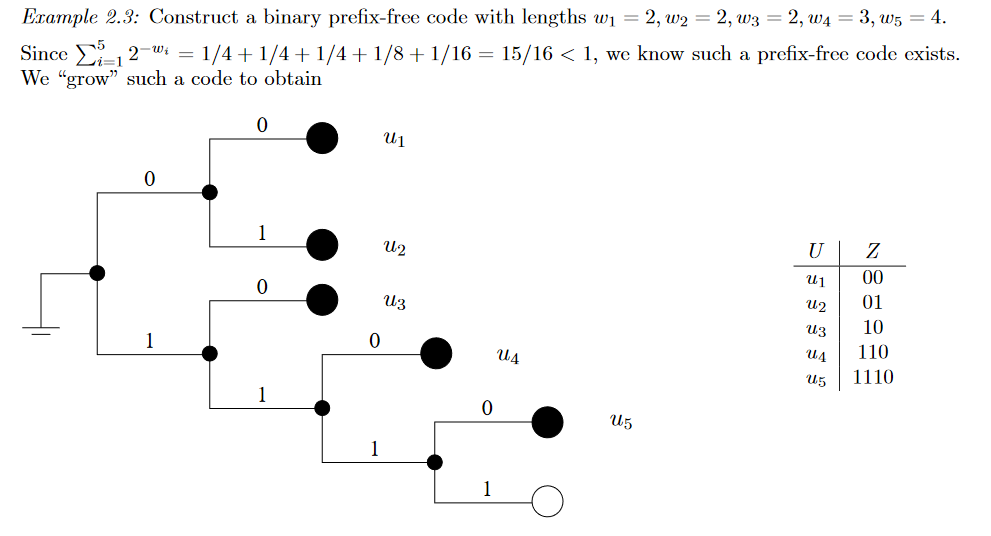
\includegraphics[width=\textwidth]{p-feg.png}

\subsection{}

Now, suppose that the source random variable $X \sim P_X$, we want to obtain a collection of integers $l_1, \cdots, l_k$ such that Kraft inequality is satisfied, then we know how to get the code for $X$.
$$ \sum_{i=1}^{k} 2^{-l} \leq 1$$
\begin{itemize}
    \item Suppose all codewords are of the same length, $$ k 2^{-l} \leq 1 \Rightarrow l \geq \log k$$

    Hence we can pick $l = \ceil{\log k}$ (ceil function). But there is no guarantee that this code is `good', it may not have small average length.

    \item We know average length $= \sum p_i l_i$.

    Then we will choose small $l_i$ for larger $p_i$. (while taking care that it satisfies Kraft inequality)
\end{itemize}

\section{Shannon-Fano code}

We fix,
\begin{equation}
    l_i = \ceil{ \log_2 \frac{1}{p_i}}
\end{equation}

 where $p_i$ is the probability of $X$ taking the $i^{th}$ value in $\mathcal{X}$.

Clearly $l_i \geq 1$.

\begin{align*}
    \sum_{i=1}^k 2^{-l_i} &= \sum_{i=1}^k 2^{-\ceil{\log_2 \frac{1}{p_i}}}  =\leq \sum_{i=1}^{k} 2^{- \log_2 \frac{1}{p_i}} \\
    &= \sum_{i=1}^k p_i = 1
\end{align*}

The lengths given by $(3)$ satisfy Kraft inequality. We can use the tree-pruning algorithm (see sec 1.3) to get a prefix-free code for $X$.

This code obtained is called as the Shannon-Fano code.

Now,

\begin{align*}
    L_{\text{Shannon-Fano}} &= \sum_{i=1}^{k} p_i \ceil{\log_2 \frac{1}{p_i}} \\
    &< \sum_{i=1}^{k} p_i \left( \log_2 \frac{1}{p_i} +1 \right) \\
    &< H(X)+1
\end{align*}

But S-F code is not always an optimal length prefix-free code.

\subsection{Example for Shannon-Fano code}
$$ X \in \mathcal{X}= \{ x_1,x_2,x_3,x_4 \}$$
\begin{equation*}
        P_X (x_i)=
        \begin{cases}
          1/4, & \text{if}\ i=1 \\
          1/2, & \text{if}\ i=2 \\
          1/9, & \text{if}\ i=3 \\
          5/36, & \text{if}\ i=4
        \end{cases}
    \end{equation*}

Lengths satisying the Kraft's inequality for the Shannon-Fano code
$$ l_i= \ceil{\log_2 \frac{1}{P_X (x_i)}}= \begin{cases}
  2, & \text{if}\ i=1 \\
  1, & \text{if}\ i=2 \\
  4, & \text{if}\ i=3 \\
  3, & \text{if}\ i=4
\end{cases} $$

$$ \bar{L}= \sum_{i=1}^{4} p_i l_i = \frac{57}{36}$$

Obtaining the Shannon-Fano code:
\begin{itemize}
    \item Arrange lengths in ascending order: $l_2 \leq l_1 \leq l_4 \leq l_3$. Hence we pick off a node at depth 2, then 1, 4 and at 3 and delete all the successors.

    \item Now we can choose the codewords from the binary tree, say
    $$ x_1 \to 01 \qquad x_2 \to 1 \qquad x_3 \to 0010 \qquad x_4 \to 000$$
    Hence, the prefix-free Shannon-Fano code is $\{ 01,1,0010,000\} $.
\end{itemize}

\section{Huffman coding}
We will show an optimal code construction that has smaller average length compared to the Shannon-Fano code.

\subsection{Lemma's}

Let us see some intuitive lemma's about an optimal code for a random variable $X$:

Assume that $X \in \mathcal{X}= \{ x_1, \cdots, x_k\}$.

$P_X(x_i)= p_i, i=1, \cdots , k$, without loss in generality, let $p_1 \geq \cdots \geq p_k$.
\begin{enumerate}
    \item Consider that $l_1, \cdots, l_k$ are the lengths of the codewords associated to the messages $x_i, i=1,\cdots, k$ respectively in any optimal code for X.

    Then,
    \begin{equation}
        l_1 \leq \cdots \leq l_k
    \end{equation}

    Proof: Suppose $\mathscr{C}$ is an optimal code in which $\exists $ some distinct $i,j \in \{1,\cdots, k \}$ such that $p_i > p_j$ but $l_i > l_j$. (Assumption of the contrary)

    We shall show that there is another code $\mathscr{C}'$ which has smaller average length $L_{\mathscr{C'}}$ than $L_{\mathscr{C}}$.

    Cosider the code $\mathscr{C}'$ in which the codewords for $x_i$ \& $x_j$ are swapped between those in $\mathscr{C}$.
    $$ \underbar{c}_{\mathscr{C'}}(x_j)=\underbar{c}_{\mathscr{C}}(x_i) \qquad \underbar{c}_{\mathscr{C'}}(x_i)=\underbar{c}_{\mathscr{C}}(x_j)$$

    Now in $\mathscr{C}$,

    $$l_{i, \mathscr{C}} :=  \text{length of codeword of } x_i \text{ in }\mathscr{C}= l_j$$
$$l_{i, \mathscr{C'}}= l_i$$

So, $l_{i, \mathscr{C'}}$ is having the same codewords as $\mathscr{C}$ and hence is also prefix-free.
$$ \bar{L}_\mathscr{C'}= \sum_{k= \{ 1, \cdots, k\} \setminus \{ i,j\}}  p_k l_k+ p_i l_i + p_j l_j$$
$$ \bar{L}_\mathscr{C}= \sum_{k= \{ 1, \cdots, k\}} p_k l_k$$
$$ \bar{L}_\mathscr{C'} - \bar{L}_\mathscr{C} = p_i(l_j -l_i)+ p_j(l_i -l_j) =(p_i-p_j)(l_j -l_i) $$

We have $p_i > p_j$, but $l_i > l_j$,
$$ \Rightarrow  \bar{L}_\mathscr{C'} - \bar{L}_\mathscr{C} < 0 \Rightarrow  \bar{L}_\mathscr{C'} < \bar{L}_\mathscr{C}$$
$\Rightarrow$ $\mathscr{C}$ is not optimal, thus this a contradiction. $(4)$ has to happen for an optimal code.

\item Consider the tree representation of a code which is optimal code. In such a tree, it should be true that either each node is a codeword or it has at least 2 successors which are codewords. i.e. There are no unused leaves in the tree of an optimal code.
%3/7

Proof: Let $\mathscr{C}$ be the optimal code. Let us consider the tree corresponding to this, suppose it has an unused leaf. Because the code is optimal, these unused leaves must be at maximum depth in the tree. Then, for at least one value $x_i$ of $\mathscr{C}$, we have the situation

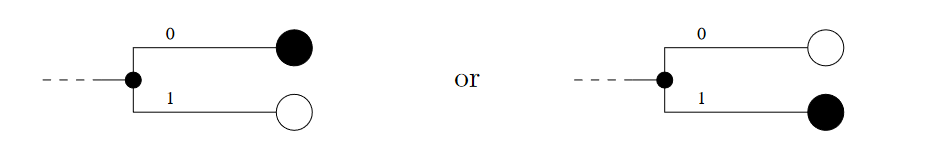
\includegraphics[width=\textwidth]{huffman.png}

In either case, we can delete the last digit of the codeword for $x_i$ (without changing the other codewords) and still have a prefix-free code. But the new code has smaller $\bar{L}$ and thus the original code could not have been optimal.

\item There is an optimal prefix-free code for random variable $X$ such that the codewords associated to the two smallest probability symbols are siblings (share the same parent). i.e. two least likely codewords differ only in their last digit.

Proof: Let $\mathscr{C}$ be some optimal code for random variable. Suppose $\mathscr{C}$ already satifies the property specified above, then we are done.

Suppose $\mathscr{C}$ doesn't satify the property, we know:

$$ l_{k-1}\leq l_k \qquad as \qquad p_{k-1} \geq p_k$$

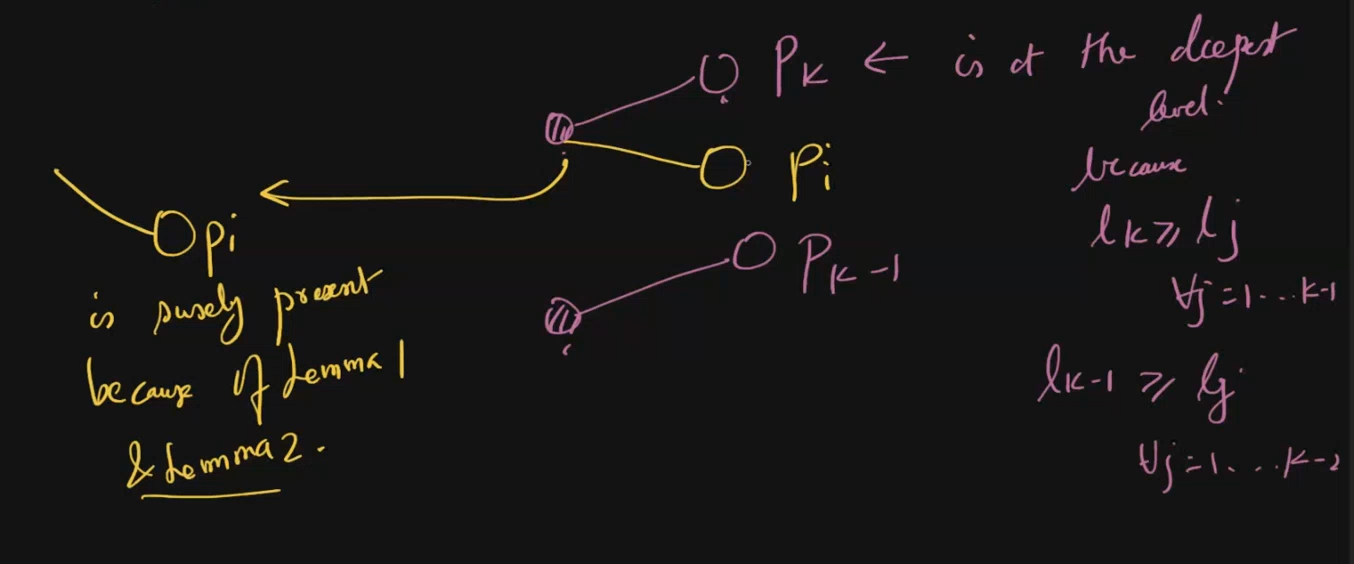
\includegraphics[width=\textwidth]{lemma3.png}

Note that $l_i = l_k$ and $i \neq k-1$.

$$ \Rightarrow l_i \leq l_{k-1} \leq l_k = l_i  \qquad \text{from Lemma-1}$$

$$ \Rightarrow l_i = l_{k-1}= l_k$$

Interchange the codewords for the $i^{th}$ and $(k-1)^{th}$ symbols and get a new code $\mathscr{C'}$.
$$ \Rightarrow \bar{L}_\mathscr{C} = \bar{L}_\mathscr{C'}$$

Now $\mathscr{C'}$ satisfies the property in Lemma 3.

\end{enumerate}

\subsection{Huffman coding}

Say we have $p_X$, assume that $p_1 \geq \cdots \geq p_k$. Unlike Shannon-Fano code, here we are building the tree in reverse. We pick $p_{k-1}$ and $p_k$ as they have the least 2 probabilities.

These are assigned to siblings in the tree and now the parent of them has probability $p_{k-1}+ p_k$.

Now we can form a new distribution using these $k-1$ probabilities (symbols) i.e. $p_1, \cdots, p_{k-2}, p_{k-1}+ p_k$. Now, if $\{ p_{k-2}, p_{k-1}+ p_k \}$ are the least 2 probabilities, a new node is assigned to $p_{k-2}$.
We repeat the process until all codewords are assigned.

\subsection{Example}

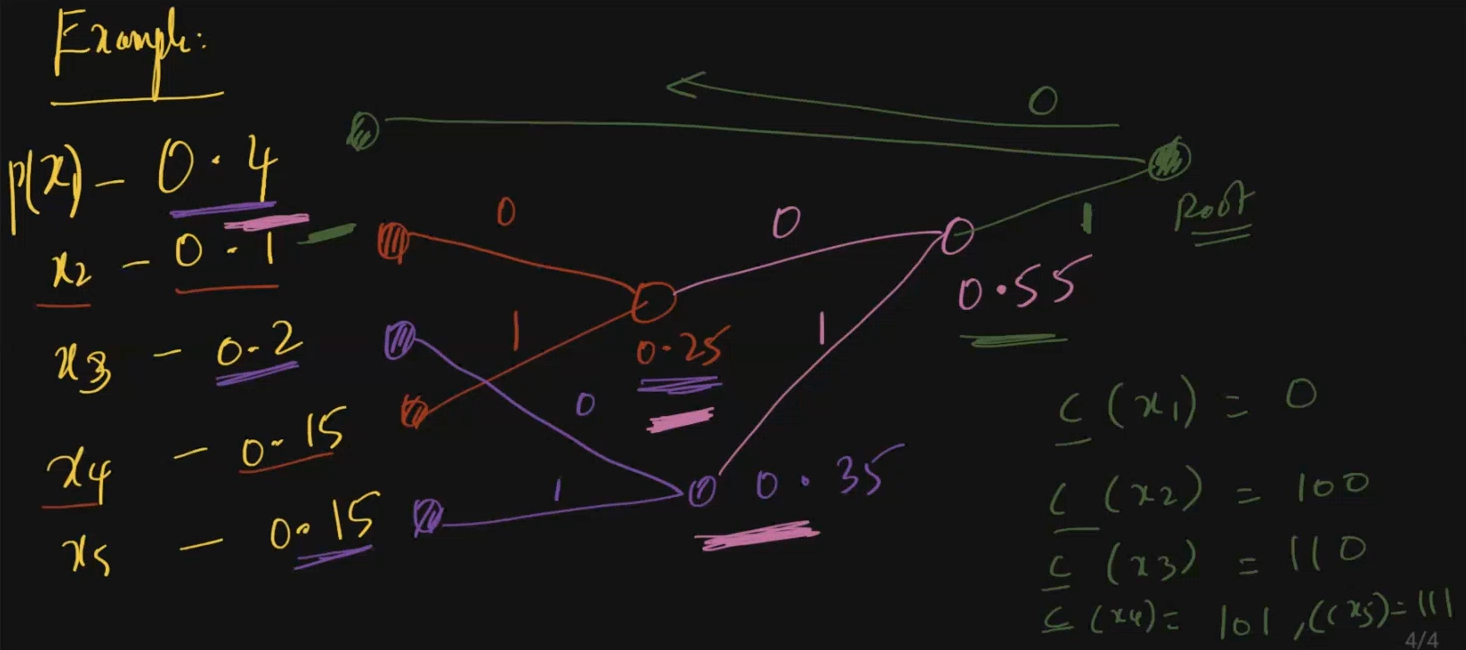
\includegraphics[width=\textwidth]{huffmaneg.png}

\end{document}
